\chapter{Unifying Logic} \label{uni}



\section{The architecture of the Semantic Web}
\begin{figure}[h!]
	\centering
	%\begin{adjustwidth}{-\marginnotewidth}{}%
	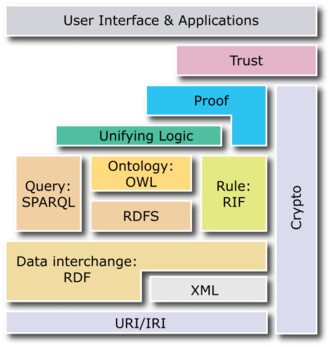
\includegraphics{Semantic_Web_Stack}
	%\end{adjustwidth}
	\caption{Semantic Web Stack in its version from 2007.}
	\label{fig:stack}
\end{figure}

To concretely realise the dream of a machine understandable Web as it was envisioned by Tim Berners-Lee et al. \cite{SemanticWeb}, 
an architecture has been proposed, the  
 ``Semantic Web Stack'' (aka ``Semantic Web Layer Cake'').
This stack provides a structural overview of the different concepts, technologies and standards needed for the Seamntic Web to become reality. 
Its shape has changed over the years \cite{Gerber2} due to the progress made---several languages such as \rdf \cite{rdf} and SPARQL \cite{sparql} have been standardised---but also 
as a consequence of controversial discussion \cite{twotowers,rearch}. 
Knowing that the current version can---and most probably will---evolve and change in the coming years, we take the current 
version\footnote{Available at: \url{https://www.w3.org/2007/03/layerCake.svg}.} 
into account and discuss its different parts. This version is displayed in Figure~\ref{fig:stack}.


% The Semantic Web as it is worked on today was introduced at the beginning of this millennium.\cite{SemanticWeb}
% Tim Berners-Lee et al. had the idea of a Semantic Web which  
% 
% Together with that proposal, there were more concrete plans, how such a vision can be realised including the discussion of the structure of such a new Semantic Web. 
% A first version of the envisioned architecture was presented by Tim Berners-Lee in the year 2000.\footnote{\url{https://www.w3.org/2000/Talks/1206-xml2k-tbl/slide10-0.html}} 
% Since then, this architecture has changed several times
% %came with a first version\footnote{\url{https://www.w3.org/2000/Talks/1206-xml2k-tbl/slide10-0.html}} 
% Together with that idea different strategies and concepts how this new Web can come into practice have been proposed.
% One of them is the Semantic Web architecture, %realize that idea an architecture was proposed\footnote{First version: \url{https://www.w3.org/2000/Talks/1206-xml2k-tbl/slide10-0.html}}  
% the ``Semantic Web Stack'' (aka ``Semantic Web Layer Cake''). Even though
% there is no official working group addressing the topic of that architecture, 
% there have been several changes from the original architecture which was proposed in a talk by Tim Berners-Lee in the year 2000.\footnote{\url{https://www.w3.org/2000/Talks/1206-xml2k-tbl/slide10-0.html}} 
% 


Introduction given by Hogan \cite{hogan}.



Gerber \cite{Gerber} \cite{Gerber2}. Really nice: abstracts from technnologies. Bad: the word ``unifying Logic'' dissapeared.

Ian Horrocks: two towers \cite{twotowers} -- by supporting the closed world assumption we get two semantic webs.


\cite{rearch} Paper by Boley, Kifer, etc. ``realistic'' architecture, not just one technology. 


\subsection{Data Interchange}
RDF

\cite{rdf}
\subsection{Querying}
\subsection{Ontologies}
RDFS
OWL

Mention: RDF is only compatible with owl full

\cite{twotowers} think that the rules and owl should not be side by side, they see the open world assumption as problem and want to have the rule layer on top of owl dl.

Maybe also mention that the connection of owl and rdfs is rather artificial -> two semantic definitions...
\subsection{Rule Based Logics}

History about big discussion open vs. closed world assumption.

Discussion: closed world assumption a problem

comes also in \cite{rearch}.

Solution:scoped negation as failure.

The paper above sees rules without negation as failure such as swrl just as extension of owl and not as belonging to the other format.

rules and owl see each other as black boxes.
we can combine them
-> this reminds me a little bit of validation where we first do dl reasoning and then querying

the paper also see querying as some kind of rule application (I think they are right here).


RIF

SWRL

N3

\cite{N3Logic}

\subsection{Unifying Logic}
Explain this unifying logic, list the attempts to find one and answer the question: why N3 and not those?



Here or somewhere else mention description logic programs \cite{DLP} which try to combine Description Logic and Logic Programming. - OK, rather their intersection.

\cite{knorr} rules as unifying logic

\cite{unilogic} first attempt to close the rift between rule-based and description logic reasoning, problem remains: open world assumption


What do we expect from the ``unifying logic''?

The vision of the Semantic Web is to enable machines to use the Web just as humans do. For that they need to be able to \emph{understand} and \emph{exchange} data through the Web. 
An unambiguous way to express knowledge is needed, a logic. 
This logic needs to be well defined to avoid misunderstandings and it needs to be agreed on this definition between all possible parties involved.


Different approaches in the ``quest for a unifying logic'': extend owl (nominal schemas, same paper \cite{unilogic}), ``merge'' owl and rules (both mentioned in \cite{unilogic}). We go a third way: rules for all.

approaches consider worst case time complexity (e.g. \cite{unilogic}). -> argue that this is nice but we focus on practical cases.

OWL and rdf is already artificial, rules are natural extension of RDF and the can cover owl.

Later on mention integrity constraints on data bases which are needed for validation.

Artikel von Motnik \cite{DLASP} sagt was ueber default rules for validation -> validation ist ein ziemlich interessantes Thema hier.

unifying logic on application level, not just a construct -> we therefore exclude owl full.

allgemein: answer set programming hat zwei Formen der Nagation.

noch was von Lifschitz und asp zitieren.


Also say why you should go for N3: unifying logic is not just a theoretical construct, it also gives practical advantages: reasoning is often faster when you use only one logic.  

somewhere: reification is not the same as citation.

Knorr hat DL style syntax
It has advantages if you need 
the features of different frameworks. Of course, if you know that, eg only querying is needed you should still go for SPARQL.


% The Unifying Logic needs to be well-defined in itself, it needs to be able to ``understand'' the underlying formats, in particular to query, do DL reasoning and use rules. 
% Additionally it should provide the opportunity to connect to the proof layer.
Requirements:
\begin{description}
 \item[clear semantic definition] 
The meaning of every statement needs to be clearly defined.
 \item[compatibility with existing Web standards]  Existing standards of the Semantic Web need to be supported. 
 In particular, querying, Description Logics, and rule based reasoning need to be covered.
 \item[support of proofs] It must be possible to express, interchange and check all derivations made in the logic.
 \item[capability to handle change] It must be possible to express and reason about change.
\end{description}
\subsection{Proofs}
\section{Research questions}
Question: Is N3 a suitable candidate to become the unifying logic for the semantic web?

Sub-questions:

Can we give a clear semantic definition of Notation3 Logic?

How does Notation3 Logic interfere with other formats? Can SPARQL, OWL and RIF be expressed?

Is it possible to express proofs in N3?

Can N3 handle change?

I think I need to be more specific. To find that: what do I actually do here?



% \textbf{Part 4: going beyond the limits}
% 
% introduce weighted transition logic to express change
% 
% This part is optional



Somewhere I need to talk about problems, especially decidability and for example the problems of OWL full.

Should I have a chapter about negation as failure?

Problem: blank nodes in SPARQL